\section{Methodology}
\subsection{Profiling SIFT}
Profiling for this project focused on two well known implementations of the SIFT algorithm, SIFT++ and VLFeat. Though initial profiling was conducted on VLFeat, SIFT++ also was used to enable easier analysis as it is less reliant on object oriented structures.

Profiling was conducted by running the sift program included with VLFeat and siftpp included with SIFT++ through Valgrind's Callgrind module. This produced outputs suitable for showing which functions were called most within the SIFT algorithm and how much time was spent in them. In both implementations, the functions handling image convolution proved to take a large portion of the run time. The VLFeat implementation, shown in Figure \ref{fig:vlfeat}, spends approximately 35\% of its running time doing image convolution. Shown in Figure \ref{fig:siftpp} is a similar measurement taken from SIFT++.  This shows that convolution a computationally dense piece of code in the two SIFT implementation.

\begin{center}
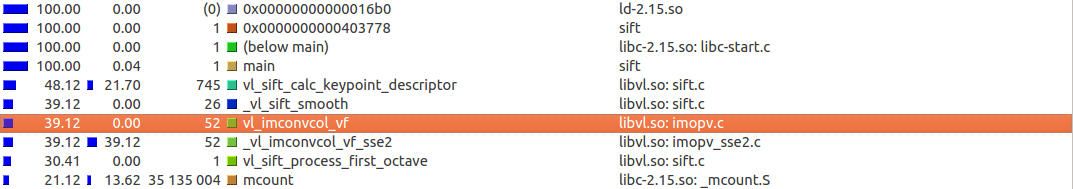
\includegraphics[width=120mm]{vlfeat.png}%
\captionof{figure}{}\label{fig:vlfeat}%
\end{center}

\begin{center}
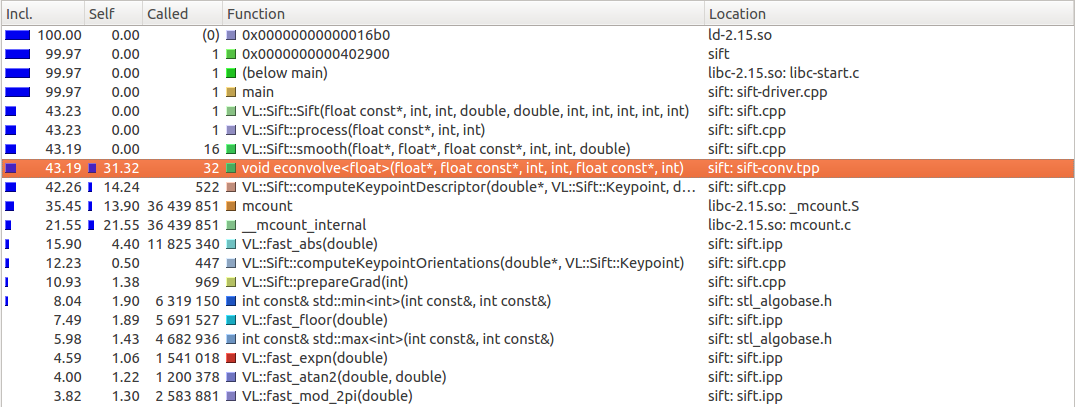
\includegraphics[width=120mm]{siftpp.png}%
\captionof{figure}{}\label{fig:siftpp}%
\end{center}

A review of both convolution implementations shows two distinct behaviors - looping and memory access. Specifically, convolution steps through each pixel in an image, requiring a nested loop resulting in a O(NM) runtime (for an NxM image). At each stage of this loop, image data is both read from and written to memory. Neither of these attributes is unusual for image processing, but they are nevertheless the most common operations within the SIFT algorithm. 

After doing this analysis, it was clear that improving memory performance and parallelizing image convolution was the primary path to achieve the necessary performance in our target application.

A simple calculation of speedup using Amdahl's Law shows that if we are able to fully parallelize the convolution, we can achieve a speedup of 1.54. 

\begin{equation*}
Speedup =\frac{1}{(1-0.35) + \frac{0.35}{\infty}} \approx 1.54
\end{equation*}

\subsection{Run time}
Running siftpp on a canonical 512x512 image yielded an average wall clock time of 1.36 seconds on an Intel Core 2 Quad Q6600. This is no where near real time performance. Certainly, some of this time is spent doing I/O operations. We tried to profile the I/O operations using strace, but did not have any success. Leaving I/O aside, we accept the fact that we can't get near real time processing of images. Therefore, a 1.54 speedup in processing would still be useful in our application.
